\chapter{Геометрия расширяющейся Вселенной}

Речь идет о расширяющейся Вселенной и ее геометрии. Цель состоит в том, чтобы описать, что значит расширение пространства, прежде чем спрашивать, что вызывает это расширение. Ньютоновская \(F=ma\) космология будет позже, и лишь после этого геометрия и динамика будут объединены в полный формализм Фридмана--Робертсона--Уокера.

\section{Сопутствующие координаты на расширяющейся прямой}

Начнем с простейшего возможного примера: одномерного пространства, а не пространства-времени. Представьте себе бесконечную прямую с равномерно расположенными на ней галактиками. Координата \(x\) пока еще не измеряет физическое расстояние. Она служит меткой для галактик. Можно думать об \(x\) как об имени галактики, и это имя остается связанным с галактикой, даже если вся конфигурация растягивается или сжимается.

Пусть физическое расстояние от галактики с меткой \(x=0\) до галактики с меткой \(x=1\) равно \(a\). Тогда физическое расстояние между любыми двумя галактиками равно
\begin{equation}
d=a\,\Delta x.
\end{equation}
Координатная разность \(\Delta x\) — это лишь разность меток. Множитель \(a\) переводит эту разность меток в действительное расстояние, измеряемое метровыми стержнями.

Теперь представьте эту прямую как упругую нить, которую растягивают. Метки остаются при галактиках, но расстояние между соседними галактиками меняется со временем. То же соотношение принимает вид
\begin{equation}
d(t)=a(t)\,\Delta x.
\end{equation}
На этом этапе однородность означает просто, что соседние галактики повсюду расположены на одинаковом расстоянии друг от друга, хотя это общее расстояние может меняться со временем.

\section{Закон Хаббла и отсутствие центра}

Чтобы найти относительную скорость двух фиксированных галактик, будем рассматривать одну и ту же пару, так что \(\Delta x\) не меняется со временем. Дифференцируя, получаем
\begin{align}
\dot d &= \dot a\,\Delta x \\
       &= \frac{\dot a}{a}\,a\,\Delta x \\
       &= \frac{\dot a}{a}\,d.
\end{align}
Если определить
\begin{equation}
H(t)\equiv \frac{\dot a}{a},
\end{equation}
то
\begin{equation}
\dot d = H(t)\,d.
\end{equation}
Это и есть закон Хаббла.

Историческое выражение ``постоянная Хаббла'' вводит в заблуждение. Эта величина постоянна в пространстве, а не во времени. В данный момент она одинакова для каждой галактики, но, вообще говоря, меняется по мере эволюции Вселенной. Ее правильнее рассматривать как параметр Хаббла.

Этот закон говорит, что более далекие галактики удаляются быстрее. Он не выделяет никакого центра. Ничто в этом рассуждении не выделяет \(x=0\) или любую другую точку. Каждый наблюдатель видит одно и то же правило. Следовательно, расширяющаяся Вселенная в этой модели не является взрывом из одного выделенного места.

Красное смещение появляется сразу. Если две галактики обмениваются световыми сигналами, удаляясь друг от друга, принятый свет смещается в красную сторону. Чем больше скорость удаления, тем больше красное смещение. Поэтому спектральные линии сообщают нам о скоростях удаления. Расстояния измерять труднее, и ранние оценки Хаббла были грубыми. Его первый график был не идеальной прямой, а разрозненным набором точек с большими неопределенностями. И все же геометрический принцип пережил этот шум: скорость удаления пропорциональна расстоянию.

\begin{classroomqa}
\audiencequestion{Если галактики достаточно далеко друг от друга, следует ли из закона Хаббла, что они движутся быстрее скорости света?}\lecturetimestamp{00:20:23}
\lecturerresponse{Да, в этом смысле удаления — да. То, что вы говорите, верно. Мы к этому обязательно вернемся. Это одна из самых важных вещей.}
\end{classroomqa}

\section{Более высокие размерности, изотропия и временная зависимость \(a(t)\)}

При добавлении большего числа пространственных измерений по существу ничего не меняется. В двух измерениях представьте квадратную решетку галактик, помеченных координатами \((x,y)\), а в трех измерениях — координатами \((x,y,z)\). Эти координаты снова являются сопутствующими метками. Они движутся вместе с галактиками, а не измеряют непосредственно физическое расстояние.

Почему расстояние в направлении \(x\) должно быть таким же, как расстояние в направлении \(y\)? Ответ дает наблюдение. Если бы галактики в одном направлении систематически располагались плотнее, чем в другом, небо выглядело бы по-разному в разных направлениях. На достаточно больших масштабах этого нет. Эта одинаковость по направлениям и есть изотропия.

В двух измерениях расстояние между двумя галактиками равно
\begin{equation}
d=a\sqrt{(\Delta x)^2+(\Delta y)^2},
\end{equation}
а в трех измерениях
\begin{equation}
d=a\sqrt{(\Delta x)^2+(\Delta y)^2+(\Delta z)^2}.
\end{equation}
Для фиксированной пары галактик координатные разности остаются постоянными, поэтому дифференцирование снова дает
\begin{equation}
\dot d=\frac{\dot a}{a}\,d.
\end{equation}
Закон Хаббла не меняется.

Однородность означает одинаковость от места к месту. Изотропия означает одинаковость от направления к направлению. Ни то ни другое не является точным на малых масштабах. Смотреть сквозь Млечный Путь — не то же самое, что смотреть вне его плоскости, и отдельные галактики на малых расстояниях распределены неравномерно. Но после усреднения по многим галактикам Вселенная на больших масштабах выглядит приблизительно одинаковой везде и во всех направлениях.

\begin{classroomqa}
\audiencequestion{Если скорость пропорциональна расстоянию и расстояние увеличивается, означает ли это, что фиксированная пара галактик обязательно должна удаляться друг от друга с ускорением?}\lecturetimestamp{00:40:22}
\lecturerresponse{Нет. Закон Хаббла говорит, что в данный момент скорость удаления пропорциональна расстоянию. Сам по себе он не говорит, увеличивается или уменьшается со временем скорость одной фиксированной пары. Это зависит от конкретной временной зависимости \(a(t)\). Если \(a(t)\propto t\), соседние галактики расходятся с постоянной скоростью. Если \(a(t)\propto t^2\), скорость удаления фиксированной пары растет со временем. Если \(a(t)\propto \log t\), она уменьшается со временем. Закон \(\dot d=(\dot a/a)d\) всегда верен как функция расстояния, но ускорение и замедление — отдельные вопросы.}
\end{classroomqa}

Долгое время космологи ожидали, что Вселенная должна расширяться с замедлением, поскольку гравитация должна тормозить начальное расширение так же, как она замедляет тело, брошенное вверх. Здесь важно лишь то, что сам по себе закон Хаббла не определяет поведение \(\dot a\) или \(\ddot a\).

\begin{classroomqa}
\audiencequestion{Как задается начальное значение масштабного фактора \(a\)?}\lecturetimestamp{00:46:18}
\lecturerresponse{Его общая нормировка произвольна. Физически важно не численное значение \(a\) само по себе, а то, как оно меняется. Если определить другой масштабный фактор \(b=3a\), то \(\dot b/b=\dot a/a\). Умножение \(a\) на постоянный множитель меняет соглашения или единицы измерения, но не параметр Хаббла.}
\end{classroomqa}

\section{От пространственной метрики к метрике пространства-времени}

Теперь заменим \(\Delta x\) на \(dx\). Физическое расстояние между соседними точками равно
\begin{equation}
ds=a\,dx,
\end{equation}
так что
\begin{equation}
ds^2=a^2\,dx^2.
\end{equation}
Это пространственная метрика в одном измерении. Коэффициент при \(dx^2\) равен
\begin{equation}
g_{xx}=a^2.
\end{equation}
Следовательно, расширяющуюся Вселенную можно описать, сказав, что пространственная часть метрики зависит от времени.

Чтобы перейти от пространства к пространству-времени, используем релятивистский интервал. В одном пространственном измерении,
\begin{equation}
d\tau^2=dt^2-a^2(t)\,dx^2.
\end{equation}
Для сопутствующего наблюдателя \(dx=0\), так что \(d\tau=dt\). Обычное космическое время — это собственное время, измеряемое часами, движущимися вместе с галактиками.

Рисунок на доске на этом этапе полезен, потому что он объединяет сопутствующие мировые линии, элемент линии и обозначения метрики.
\begin{figure}[H]
\centering
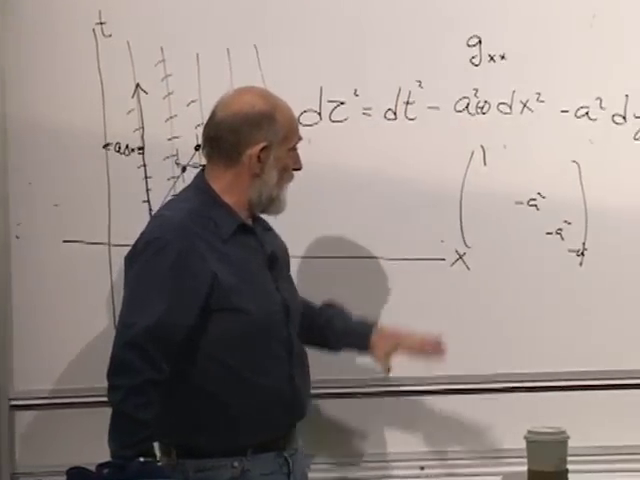
\includegraphics[width=0.82\textwidth]{lecture_01_figure_02.png}
\caption{Сопутствующие мировые линии в расширяющейся одномерной Вселенной вместе с соответствующим интервалом пространства-времени.}
\end{figure}

В трех пространственных измерениях тот же образец дает осторожное обобщение\footnote{Доска частично закрыта в районе 00:56:38--00:58:51. Эта трехмерная форма следует из устного перехода от одного пространственного измерения к трем вместе с видимой на доске диагональной структурой.}
\begin{equation}
d\tau^2=dt^2-a^2(t)\bigl(dx^2+dy^2+dz^2\bigr),
\end{equation}
с диагональной метрикой
\begin{equation}
g_{\mu\nu}=\mathrm{diag}\bigl(1,-a^2,-a^2,-a^2\bigr).
\end{equation}
Внедиагональные члены обращаются в нуль,
\begin{equation}
g_{tx}=g_{ty}=g_{tz}=0.
\end{equation}

Однородность означает, что коэффициенты метрики могут зависеть от времени, но не от пространственного положения. Изотропия означает, что все три пространственных направления входят одинаковым образом.

\begin{classroomqa}
\audiencequestion{Разве не следует думать об \(dx\) как о расстоянии?}\lecturetimestamp{01:01:18}
\lecturerresponse{Нет. \(dx\) — это не расстояние. \(a\,dx\) — это расстояние. \(dx\) — всего лишь интервал меток. Полезно думать об этом так: представьте, что в некоторый момент кто-то проводит координатную сетку через галактики, а затем требует, чтобы она следовала за ними. Координатное разделение по построению остается фиксированным, тогда как физическое расстояние меняется. Можно было бы поместить единицы длины в \(x\), а не в \(a\); это вопрос соглашения. Важно произведение \(a\,dx\).}
\end{classroomqa}

\begin{classroomqa}
\audiencequestion{Коэффициент при \(dt^2\) в метрике равен \(1\). Это тоже просто вопрос соглашения?}\lecturetimestamp{01:03:24}
\lecturerresponse{Да. Само по себе здесь никакой физики нет. Если бы коэффициент зависел только от времени, можно было бы изменить временную переменную так, чтобы он стал просто \(dt^2\). Точно так же можно выбрать единицы, в которых \(c=1\). Что здесь не является вопросом соглашения, так это то, что этот коэффициент не зависит от положения, хотя может зависеть от времени.}
\end{classroomqa}

\begin{classroomqa}
\audiencequestion{Если подставить это в уравнения поля Эйнштейна, что получится для тензора энергии-импульса?}\lecturetimestamp{01:05:59}
\lecturerresponse{Это следующий тип вопроса, но он относится к динамике, а не к нынешнему обсуждению. Можно подставить эту метрику в уравнения Эйнштейна и спросить, какое распределение энергии-импульса сделало бы её решением. Это очень важно, но пока предметом является геометрия, а не динамика.}
\end{classroomqa}

\section{Что скрывает горизонт}

Крупномасштабную Вселенную рассматривают как однородную и изотропную лишь приближённо. Она, конечно, не однородна в масштабе звёзд, планет или даже отдельных галактик. И в каждом локальном наблюдении она тоже не является в точности изотропной.

Поле фермера хорошо передаёт правильную зависимость от масштаба. В одном масштабе оно выглядит регулярным; в гораздо меньшем — явно нет; а в масштабе, превышающем всё поле целиком, оно снова перестаёт выглядеть однородным. В космологии то же самое. После усреднения по множеству галактик крупномасштабное распределение выглядит примерно равномерным. На достаточно малых масштабах — нет.

Вселенная больше той части, которую мы можем видеть, и больше той части, которую мы вообще когда-либо сможем увидеть. В тех масштабах, которые действительно можно исследовать, она изотропна и однородна, за исключением локальных вариаций. За этими пределами нет прямого наблюдательного подтверждения.

\begin{classroomqa}
\audiencequestion{Вы сказали, что мы на самом деле никогда не узнаем этого напрямую. Означает ли это, что может существовать косвенный способ это выяснить?}\lecturetimestamp{01:10:34}
\lecturerresponse{Возможно. Сегодня большинство склоняется к мысли, что на достаточно больших масштабах Вселенная неоднородна, и я сам думаю так же. Но это ставка, которую я никогда не выиграю и никогда не проиграю, потому что по фундаментальным, самым базовым причинам мы не сможем видеть намного дальше, чем видим сейчас. Это связано с существованием горизонта.}
\end{classroomqa}

\begin{classroomqa}
\audiencequestion{Разве нельзя использовать гравитацию, чтобы искать массы за пределами того, что видно?}\lecturetimestamp{01:11:53}
\lecturerresponse{Нет. Далёкая масса может просто ввести нас в свободное падение. Сидя в закрытой комнате, мы находимся в гравитационном поле Солнца и обращаемся вокруг него, но, не видя наружу, невозможно простым способом установить, что Солнце существует. Его выдают только приливные силы, а если источник достаточно далёк, эти приливные эффекты могут оказаться слишком малы, чтобы их обнаружить.}
\end{classroomqa}

Следовательно, горизонт является предельным барьером для непосредственного знания. Он даже утверждает, почти с полной уверенностью, что Вселенная по объёму по меньшей мере в тысячу раз больше области, которую мы когда-либо сможем увидеть, и оставляет обоснование этого утверждения на потом.

\section{Ограниченное, но без границы}

Теперь перейдём к замкнутым геометриям. Бесконечная прямая открыта и неограниченна. Отрезок ограничен в том смысле, что имеет лишь конечную протяжённость. Ограниченность не означает наличия границы, а означает конечную протяжённость.

Куб со стенками не подойдёт. Он нарушает однородность, потому что человек возле стены не эквивалентен человеку далеко от стены, и нарушает изотропию, потому что даже человек в центре видит разное в разных направлениях.

Внутренность круга или шара тоже не годится. Тот, кто находится в центре, видит одно и то же во всех направлениях, но эта симметрия принадлежит только одной особой точке. Стоит отойти от центра, и в одном направлении стена близко, а в другом далеко. Тогда пространство не является ни однородным, ни изотропным для произвольных наблюдателей.

В качестве рабочего предположения на очень больших масштабах принимается, что Вселенная однородна и изотропна. Это космологический принцип. Он полезен, но не застрахован от пересмотра.

\begin{classroomqa}
\audiencequestion{Влечёт ли изотропия всюду однородность?}\lecturetimestamp{01:18:57}
\lecturerresponse{Да. Если каждый наблюдатель видит одно и то же во всех направлениях, это влечёт однородность. Но обратное неверно. Сама по себе однородность не влечёт изотропии. Вселенная может быть однородной и всё же иметь выделенное направление, например если бы она была заполнена стрелками, все из которых указывают в одну и ту же сторону.}
\end{classroomqa}

Правильная ограниченная модель — это поверхность сферы без каких-либо особенностей. Двумерное существо, существующее только на этой поверхности, обнаружит, что всякое место локально похоже на любое другое, а всякое направление — на любое другое, хотя мир конечен. Это ограниченность без границы.

\section{Замкнутая одномерная вселенная на окружности}

Чтобы сохранить алгебру простой, сведём пример со сферой к одному пространственному измерению: к жизни на окружности. В одном измерении изотропия означает, что лево и право эквивалентны. Окружность обладает именно этим свойством. Выберем одну точку и положим, что в ней \(\theta=0\). Каждая другая точка задаётся угловой координатой \(\theta\), измеряемой в радианах. Точку совсем рядом с началом, по одну его сторону, можно описать либо малым отрицательным углом, либо углом, чуть меньшим \(2\pi\). Эта периодичность — часть геометрии.

Обитателям окружности доступна сама окружность, а не внешний радиус или центр. Они могут измерить полное расстояние по кругу, идя вдоль неё, пока не вернутся в ту же точку. Если нарисовать окружность во вмещающей плоскости, можно также ввести величину наподобие радиуса, но она относится к картине вложения, а не к внутренней геометрии, которую они измеряют.

Рисунок на доске здесь полезен, потому что на нём угловые метки и полная длина окружности показаны на одном и том же изображении.
\begin{figure}[H]
\centering
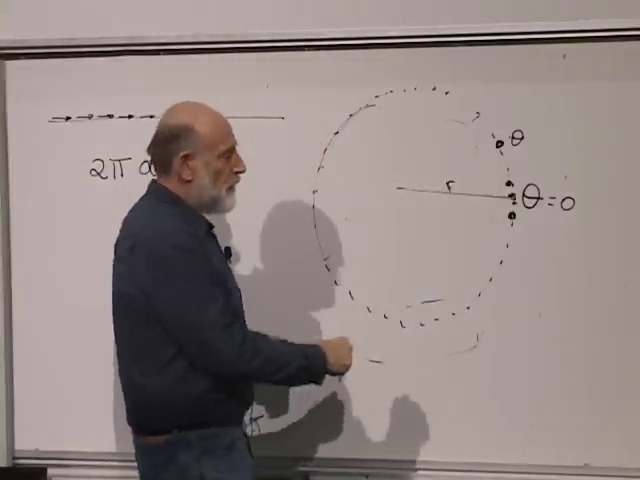
\includegraphics[width=0.82\textwidth]{lecture_01_figure_03.png}
\caption{Угловое описание замкнутой одномерной вселенной с полной длиной окружности \(2\pi a\).}
\end{figure}

Удобно принять следующее обозначение\footnote{Около 01:26:40--01:29:20 обозначения ненадолго переходят от того, чтобы принимать саму полную длину окружности за масштабный фактор, к записи её как \(2\pi a\). Здесь используется второй вариант, потому что именно он входит в формулу длины дуги.}:
\begin{equation}
L=2\pi a,
\end{equation}
где \(L\) — полная длина окружности.

Для малого углового расстояния \(\Delta\theta\) физическое расстояние равно
\begin{equation}
d=a\,\Delta\theta.
\end{equation}
Переходя к бесконечно малым, получаем
\begin{equation}
ds=a\,d\theta,
\end{equation}
и, следовательно,
\begin{equation}
ds^2=a^2\,d\theta^2.
\end{equation}
Это локальная метрика на окружности.

Если \(a\) зависит от времени, замкнутая одномерная вселенная расширяется или сжимается. Для фиксированной пары галактик,
\begin{equation}
d(t)=a(t)\,\Delta\theta,
\end{equation}
следовательно,
\begin{equation}
\dot d=\dot a\,\Delta\theta
      =\frac{\dot a}{a}\,d.
\end{equation}
Закон Хаббла сохраняется и здесь, по крайней мере для пар, которые не настолько далеко разнесены, чтобы путь вокруг окружности в другую сторону стал неоднозначным.

Метрика пространства-времени принимает вид
\begin{equation}
d\tau^2=dt^2-a^2(t)\,d\theta^2.
\end{equation}
Если величина \(a\) постоянна, пространственно-временная картина представляет собой цилиндр. Если \(a\propto t\), получается конус. Если \(a(t)\) меняется более нерегулярно, рисунок становится похожим на вазу.

Если прокрутить картину назад, галактики будут оказываться всё ближе и ближе друг к другу. Если бы по окружности было \(360\) галактик, в поздние времена они были бы хорошо разнесены, раньше — очень близко друг к другу, а ещё раньше — ещё ближе. В конце концов это были бы уже не отдельные галактики, а ещё раньше — даже не отдельные атомы. Но в пространстве по-прежнему нет никакой особой точки.

Это самый ясный ответ на вопрос о том, где в этой модели произошёл Большой взрыв. Когда \(a(t)\to 0\), каждое расстояние \(a(t)\,\Delta\theta\) стремится к нулю. Вся Вселенная сжимается повсюду одновременно. Галактики не разлетаются из одного привилегированного места во внешнем пространстве. Меняется масштаб самой геометрии. В этом смысле ответ таков: везде.

\begin{classroomqa}
\audiencequestion{Вы сказали, что пространство-время искривлено. А если это цилиндр, оно искривлено?}\lecturetimestamp{01:38:04}
\lecturerresponse{Нет. Если бы это был цилиндр, оно не было бы искривлено. Это тот случай, когда величина \(a\) постоянна во времени. Оно выглядит искривлённым только потому, что нарисовано в пространстве большей размерности. Если его разрезать, его можно развернуть на плоскость без растяжения.}
\end{classroomqa}

После этого обсуждение переходит к конусу. Если \(a\propto t\), пространственно-временная картина — конус. Вне его вершины конус тоже плоский в том же внутреннем смысле: его можно развернуть в плоскость. Вершина отличается. Это коническая сингулярность.

Следующий шаг — геометрия сферической вселенной, а затем динамика, определяющая, как \(a(t)\) растёт или уменьшается.
